\documentclass{article}
\usepackage[utf8]{inputenc}
\usepackage{graphicx}
\usepackage{wrapfig}
\usepackage{array}
\usepackage{siunitx}

\title{ELP Experiment 1}
\author{Aditya Agrawal \\ 2021AM10198 }
\date{April 2, 2022}

\begin{document}

\maketitle
\tableofcontents
\newpage
\section{Voltage Measurement}
\subsection{Aim}
To use DSO to measure the Voltage of given waveform
\subsection{Apparatus}
\begin{enumerate}
    \item{Digital Storage Oscilloscope}
    \item{DC Power Supply}
    \item{Function Generator}
    \item{Resistors and Capacitors}
    \item{Connecting Wires}
\end{enumerate}
\subsection{Theory}
\begin{equation}
    {V_{P-P}}= Deflection \times \frac{Volts}{Division} 
\end{equation}
\begin{equation}
    {V_{RMS}}= \frac{V_{P-P}}{2 \sqrt{2}}
\end{equation}
\subsection{Observation}
\begin{center}
\begin{tabular}{|c|c|c|c|}
\hline
    Deflection & $ \frac{Volts}{Division} $ &$ V_{P-P} $ & $ V_{RMS} $ \\
    \hline 
    6 & 2.00 & 11.3 & 3.99 \\
    4 & 2.00 & 8.40 & 2.97 \\ 
    3 & 2.00 & 5.68 & 1.41 \\ 
    7 & 2.00 & 14.00 & 4.95 \\
\hline
\end{tabular}
\end{center}
\subsection{Conclusion}
Hence, we were able to measure the amplitude voltage of a given sine wave signal
with the help of a Digital Storage Oscilloscope.
\newpage

\section{Frequency Measurement}
\subsection{Aim}
To study the basic working of Digital Storage Oscilloscope (DSO) and to make frequency measurement by means of Lissajous patterns. 

\subsection{Apparatus}
\begin{enumerate}
    \item Digital Storage Oscilloscope (DSO1052B)
    \item DC Power supply (0 – 30 Volts)
    \item Function Generator (0 – 3 MHz)
\end{enumerate}

\subsection{Theory}
\begin{wrapfigure}{R}{0.3\textwidth}
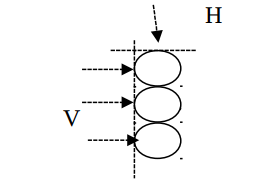
\includegraphics[width=0.25\textwidth]{2Theory.png}
\end{wrapfigure}
The unknown frequency signal is usually applied to the vertical terminal of the
oscilloscope and the standard frequency signal is applied to the horizontal amplifier. The horizontal time-base mode should be set to XY mode. Once the
DSO gets the two signals – the known and the unknown, the Lissajous pattern observed is evaluated.
\begin{equation}
    F_{Unknown}=F_{Known} \times \frac{T_H}{T_V}
\end{equation}
\begin{center}
$T_H$ is the number of points of horizontal tangency \\
$T_V$ is the number of points of vertical tangency \\
$F_{Known}$ is the known frequency\\
\end{center}
\vfill

\subsection{Observation}
\vspace{10px}
\newcolumntype{V}{>{\centering\arraybackslash} m{.4\linewidth} }
\begin{center}
\begin{tabular}{|V|c|c|c|c|} 
 \hline
    Lissajous pattern & $T_{H}$& $T_{V}$ & $F_{Known}(in kHz)$ & $F_{Unknown}(in kHz)$ \\     
    \hline
    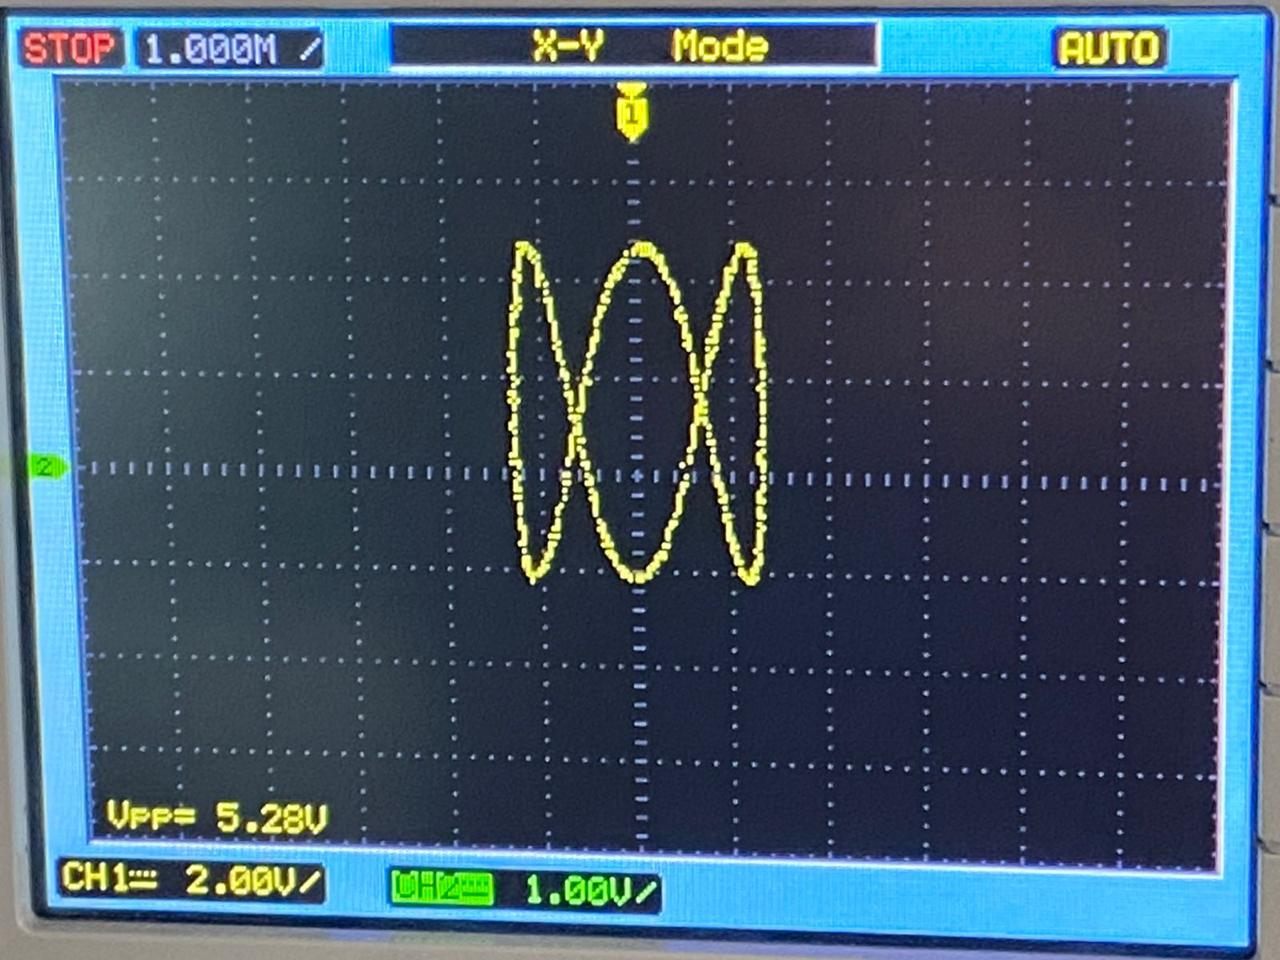
\includegraphics[width=0.25\textwidth]{part2 img1.jpeg} & 3 & 1 & 1 &3 \\
    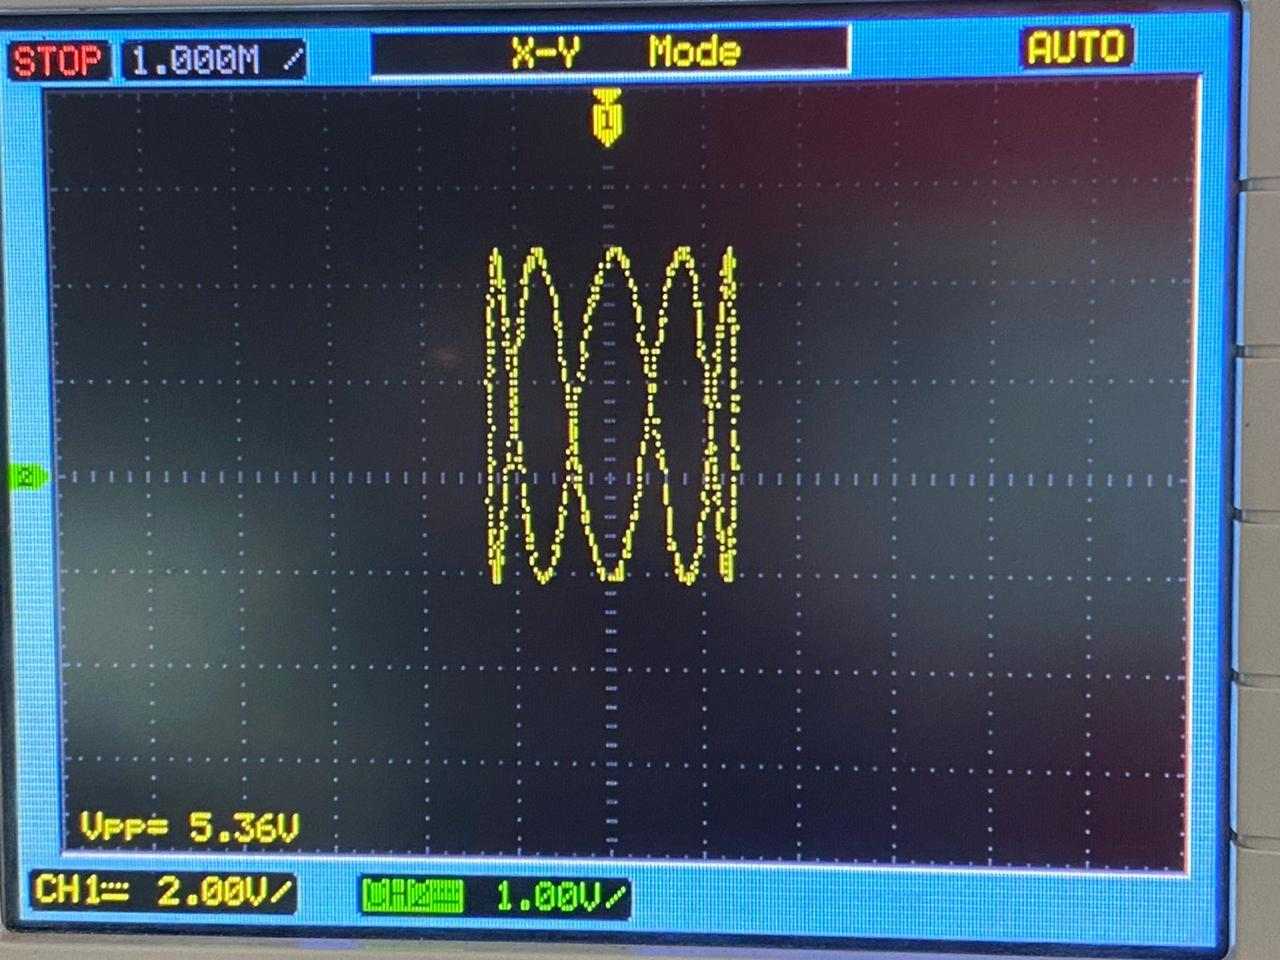
\includegraphics[width=0.25\textwidth]{part2 img2.jpeg} & 5 & 1 & 1 &5 \\
    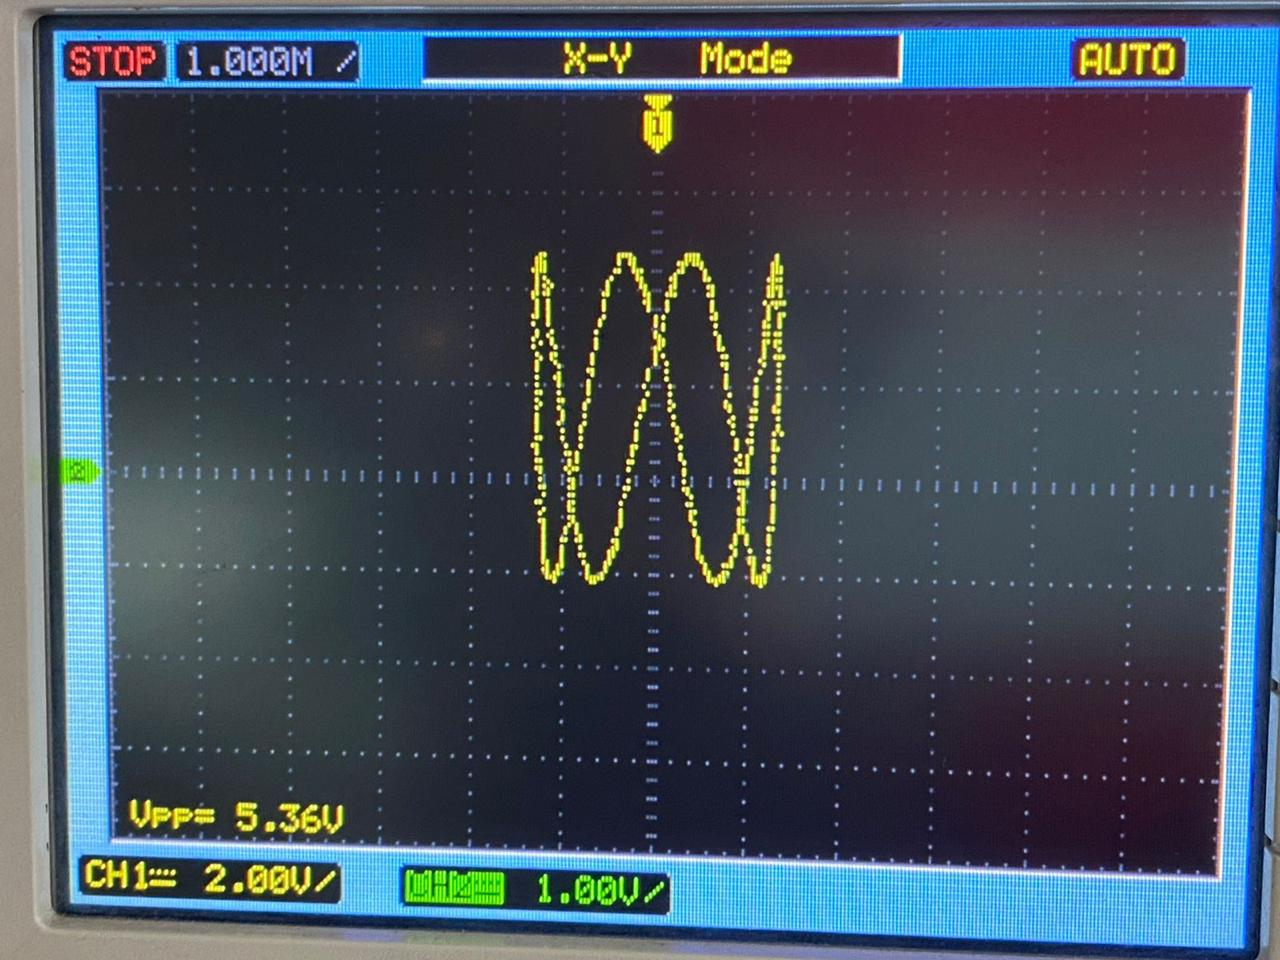
\includegraphics[width=0.25\textwidth]{part2 img3.jpeg} & 4 & 1 & 1 &4 \\
    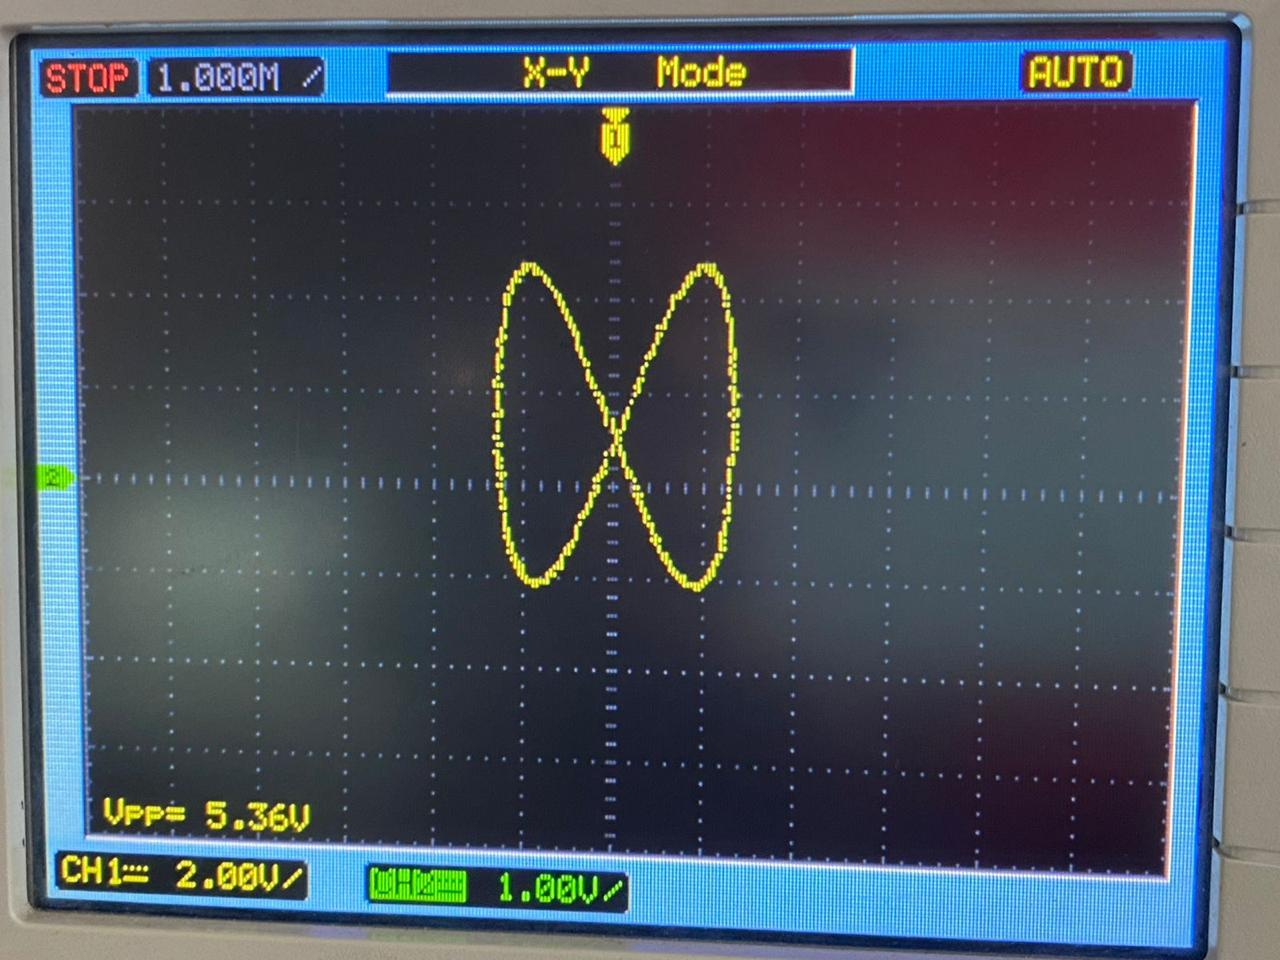
\includegraphics[width=0.25\textwidth]{part2 img4.jpeg} & 2 & 1 & 1 &2 \\
 \hline
\end{tabular}
\end{center}
\subsection{Conclusion}
Hence, we were able to study the basic working of Digital Storage Oscilloscope (DSO) and to make frequency measurement by means of Lissajous patterns.
\newpage

\section{Phase Measurement}
\subsection{Aim}
To measure the phase difference between two signals of the same frequency.

\subsection{Apparatus}
\begin{enumerate}
    \item Digital Storage Oscilloscope (DSO1052B)
    \item DC Power supply (0 – 30 Volts)
    \item Function Generator (0 – 3 MHz)
    \item Multimeter (FLUKE 115)
    \item Variable resistor
    \item Capacitor
    \item Breadboard
    \item Jumpers
\end{enumerate}

\subsection{Theory}
\begin{wrapfigure}{R}{0.2\textwidth}
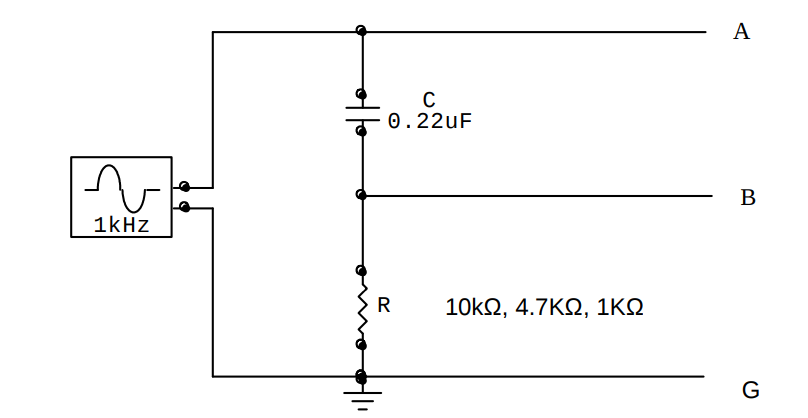
\includegraphics[width=0.4\textwidth]{3Theory.png}
\end{wrapfigure}
According to the circuit, there are two signals that are generated – the first is the one across A and G, the second is across B and G. Let us call these set of signals as Signal A and Signal B. Switching the DSO into the X-Y mode, we get ellipses.
\begin{wrapfigure}{R}{0.15\textwidth}
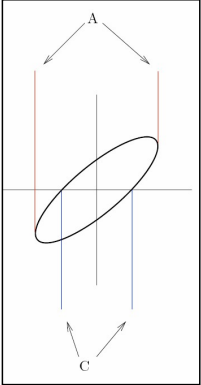
\includegraphics[width=0.15\textwidth]{3.1 Theory.png}
\end{wrapfigure}

According to the figure, the phase difference $\theta$ is given by the
equation:
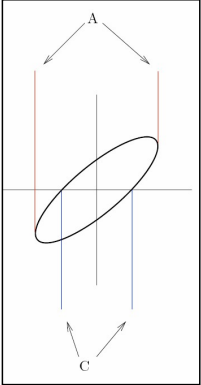
\includegraphics[width=0\textwidth]{3.1 Theory.png}
\begin{equation}
    sin  \ \theta = \frac{C}{A}
\end{equation}

Theoretically, \[ tan \theta = \frac{X_C}{R}\] where $ X_C$ is the capacitive resistance of Capacitor, given by \[ X_C = \frac{1}{\omega \times Capacitance}\]
\vfill

\subsection{Observation}
Capacitance= 0.23 µ \\
Frequency= 1 kHz \\
$X_C$= 692.33 \si{\ohm}
\vspace{10px}

\begin{center}
\begin{tabular}{|V|c|c|c|c|c|} 
 \hline
    Lissajous pattern & R(in ohms) &  A & C & $\theta $ & Calculated Value of $\theta$ \\     
    \hline
    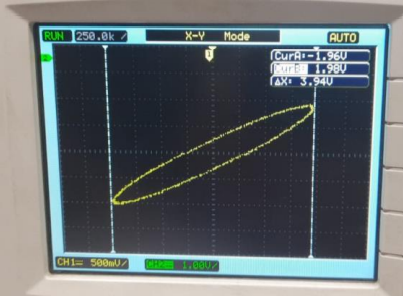
\includegraphics[width=0.25\textwidth]{img2.png} & 2.266 & 3.94& 1.18 & 0.3042 & 0.2965 \\
    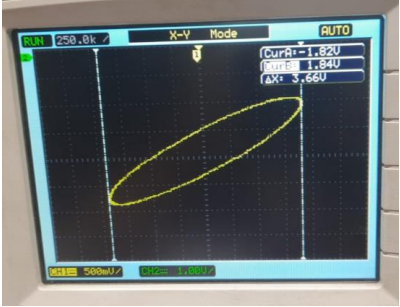
\includegraphics[width=0.25\textwidth]{img1 .png} & 1.34 &  3.67 & 1.72 & 0.4881 & 0.4678 \\
    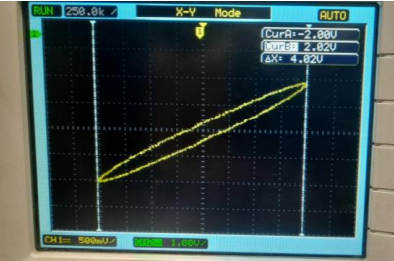
\includegraphics[width=0.25\textwidth]{img3.png} & 4.21 & 4.00 & 0.68 & 0.1708 & 0.1629 \\
    
 \hline
\end{tabular}
\end{center}

\subsection{Conclusion}
Hence, we were able to study the basic working of Digital Storage Oscilloscope (DSO) and to measure phase difference between two signals by use of Lissajous Patterns observed on the DSO screen.

\newpage
\section{Sources of Error}
\begin{itemize}
    \item Scale of DSO not properly set
    \item Loose connections
    \item Connections changed while circuit is powered
    \item Resistance in wires and change due to temperature
\end{itemize}
\section{Precautions}

\begin{itemize}
    \item Make the connections neat and tight
    \item Don’t leave the switch on for long continuous periods of time.
    \item Wear proper shoes and use insulated tools
\end{itemize}

\section{Concluding Remarks}
In this experiment, we learned how to use the DSO's(Digital Storage Oscilloscope) basic functions. The DSO was used to determine the voltage of an input sin wave signal from an FPG (Frequency Pulse Generator), as well as the frequency difference between two signals. Using the tangent approach is a good way to go. The DSO was also used to determine the phase difference between two signals, on an AC circuit, and the results were confirmed using theoretical formulae. Furthermore, we became acquainted with the fundamental functions of an oscilloscope, learned more about Lissajous Patterns, and learned how to use an oscilloscope know how to build a breadboard prototype circuit. \\
Hence we were able to analyze the theoretical knowledge gained via simple experiments using an oscilloscope.

\end{document}